\documentclass[11pt,letterpaper]{article}

\newcommand{\curso}{Algoritmos y Estructuras de Datos}
\newcommand{\tituloinforme}{Tarea 1: Análisis asintótico y Dividir para conquistar}
\newcommand{\programa}{Doctorado en Inteligencia Artificial}
\newcommand{\integrantes}{Paula Vásquez-Henríquez \\ & Guillermo Zieballe Jarpa}
\newcommand{\profesor}{Cecilia Hernández}
\newcommand{\fecha}{13 de octubre de 2026}

% ============================================================
%  Preámbulo: paquetes, estilo y macros del informe
% ============================================================

% --- Idioma y codificación ---
\usepackage[utf8]{inputenc}
\usepackage[T1]{fontenc}
\usepackage[spanish,es-noshorthands,es-tabla]{babel}
\usepackage{lmodern}
\usepackage{microtype}

% --- Página ---
\usepackage[margin=2.5cm]{geometry}
\usepackage{fancyhdr}
\usepackage{titlesec}
\setlength{\parskip}{0.5em}
\setlength{\parindent}{0pt}

% --- Matemática ---
\usepackage{amsmath,amssymb,amsthm,mathtools}
\usepackage{bm}

% --- Algoritmos (pseudocódigo) ---
\usepackage[ruled,vlined,linesnumbered,spanish,onelanguage]{algorithm2e}

% --- Código Python ---
\usepackage{listings}
\usepackage{xcolor}

% --- Figuras, tablas y árboles de recursión ---
\usepackage{graphicx}
\usepackage{booktabs}
\usepackage{array}
\usepackage{float}
\usepackage{enumitem}
\usepackage{caption}
\usepackage{subcaption}
\usepackage{tikz}
\usetikzlibrary{trees,positioning,arrows.meta,calc}
\usepackage{forest}

% --- Cajas para resultados ---
\usepackage[most]{tcolorbox}

% --- Enlaces (cargar al final) ---
\usepackage[hidelinks]{hyperref}
\usepackage[nameinlink,spanish]{cleveref}

\graphicspath{{figuras/}}

% ============================================================
%  Encabezado y pie
% ============================================================
\pagestyle{fancy}
\fancyhf{}
\fancyhead[L]{\small\curso}
\fancyhead[R]{\small\tituloinforme}
\fancyfoot[C]{\thepage}
\renewcommand{\headrulewidth}{0.4pt}

\titleformat{\section}{\Large\bfseries}{\thesection}{0.8em}{}
\titleformat{\subsection}{\large\bfseries}{\thesubsection}{0.8em}{}

% ============================================================
%  Estilo para código Python
% ============================================================
\definecolor{codefondo}{RGB}{247,247,247}
\definecolor{codeclave}{RGB}{0,80,160}
\definecolor{codecoment}{RGB}{110,110,110}
\definecolor{codetexto}{RGB}{160,40,40}
\definecolor{codenum}{RGB}{150,150,150}

\lstdefinestyle{python}{
  language=Python,
  backgroundcolor=\color{codefondo},
  basicstyle=\ttfamily\small,
  keywordstyle=\color{codeclave}\bfseries,
  commentstyle=\color{codecoment}\itshape,
  stringstyle=\color{codetexto},
  numbers=left,
  numberstyle=\tiny\color{codenum},
  numbersep=8pt,
  frame=single,
  rulecolor=\color{black!15},
  breaklines=true,
  showstringspaces=false,
  tabsize=4,
  columns=fullflexible,
  keepspaces=true,
  xleftmargin=1.5em,
  framexleftmargin=1.5em,
  % Acentos y ñ dentro del código
  literate=
    {á}{{\'a}}1 {é}{{\'e}}1 {í}{{\'i}}1 {ó}{{\'o}}1 {ú}{{\'u}}1
    {Á}{{\'A}}1 {É}{{\'E}}1 {Í}{{\'I}}1 {Ó}{{\'O}}1 {Ú}{{\'U}}1
    {ñ}{{\~n}}1 {Ñ}{{\~N}}1 {ü}{{\"u}}1 {¿}{{?`}}1 {¡}{{!`}}1
}
\lstset{style=python}
\renewcommand{\lstlistingname}{Código}

% ============================================================
%  Macros de notación asintótica
% ============================================================
\newcommand{\T}[1]{\Theta\!\left(#1\right)}
\newcommand{\Oh}[1]{O\!\left(#1\right)}
\newcommand{\Om}[1]{\Omega\!\left(#1\right)}
\newcommand{\oh}[1]{o\!\left(#1\right)}
\newcommand{\om}[1]{\omega\!\left(#1\right)}
\newcommand{\N}{\mathbb{N}}
\newcommand{\R}{\mathbb{R}}
\DeclarePairedDelimiter{\ceil}{\lceil}{\rceil}
\DeclarePairedDelimiter{\floor}{\lfloor}{\rfloor}
\DeclarePairedDelimiter{\norma}{\lVert}{\rVert}

% ============================================================
%  Entornos teóricos
% ============================================================
\theoremstyle{definition}
\newtheorem{definicion}{Definición}[section]
\newtheorem{proposicion}{Proposición}[section]
\newtheorem{lema}{Lema}[section]
\theoremstyle{remark}
\newtheorem*{observacion}{Observación}
\renewcommand{\qedsymbol}{$\blacksquare$}

% ============================================================
%  Estructura de cada ejercicio
% ============================================================
% Enunciado del ejercicio
\newtcolorbox{enunciado}{
  colback=black!3, colframe=black!35, boxrule=0.5pt, arc=2pt,
  left=6pt, right=6pt, top=4pt, bottom=4pt,
  fonttitle=\bfseries, title=Enunciado
}
\newcommand{\paso}[2]{\par\medskip\noindent\textbf{Paso #1. #2.}\par\nopagebreak[4]}

% Resultado final destacado
\newtcolorbox{resultado}{
  colback=blue!4, colframe=blue!50!black, boxrule=0.6pt, arc=2pt,
  left=6pt, right=6pt, top=4pt, bottom=4pt,
  fonttitle=\bfseries, title=Resultado
}

% Intuición / comentario pedagógico
\newtcolorbox{intuicion}{
  colback=green!4, colframe=green!40!black, boxrule=0.5pt, arc=2pt,
  left=6pt, right=6pt, top=4pt, bottom=4pt,
  fonttitle=\bfseries, title=Intuición
}


\begin{document}

\begin{titlepage}
  \thispagestyle{empty}
  \centering

  \begin{flushleft}
    
\includegraphics[height=0.9cm]{logos/Logo_UdeC.png}\hspace{4pt}%
    
\includegraphics[height=0.9cm]{logos/Logo_UBB.png}\hspace{4pt}%
    
\includegraphics[height=0.9cm]{logos/Logo_UCSC.png}\hspace{4pt}%
    
\includegraphics[height=0.9cm]{logos/Logo_UTFSM.png}\hspace{6pt}%
    
\includegraphics[height=0.75cm]{logos/Logo_GORE.png}
  \end{flushleft}

  \vspace*{3cm}

  {\large\scshape \programa\par}
  \vspace{0.4cm}
  {\large \curso\par}

  \vspace{2.5cm}
  \rule{\linewidth}{0.6pt}\par\vspace{0.4cm}
  {\LARGE\bfseries \tituloinforme\par}
  \vspace{0.3cm}
  \rule{\linewidth}{0.6pt}\par

  \vfill
  \begin{tabular}{rl}
    \textbf{Integrantes:} & \integrantes \\[4pt]
    \textbf{Profesora:}   & \profesor \\[4pt]
    \textbf{Fecha:}       & \fecha
  \end{tabular}
  \vspace{2cm}
\end{titlepage}


\tableofcontents
\newpage

\section{Actividad 1: complejidad temporal de algoritmos iterativos}
\label{sec:act1}

En esta actividad obtenemos, para cada algoritmo, una expresión para su costo y una cota
$\Theta$ ajustada.

\subsection{Algoritmo A}
\label{sec:act1a}

\begin{enunciado}
\begin{lstlisting}[language={}, numbers=none, frame=none, backgroundcolor={}]
Procedure A(n)
    for i = 1 to n
        j = i
        while j <= n
            Operation()        // costo Theta(1)
            j = 2*j
\end{lstlisting}
\begin{enumerate}[label=(\alph*)]
  \item Determine cuántas veces se ejecuta \texttt{Operation()} para un valor fijo de $i$.
  \item Escriba una sumatoria que represente el número total de ejecuciones.
  \item Obtenga una cota $\Theta$ ajustada. Se recomienda considerar, de manera
        alternativa, cuántos valores de $i$ pueden ejecutar la iteración $k$ del ciclo while.
  \item Explique por qué concluir $\T{n\log n}$ únicamente porque existe un for y un
        while sería incorrecto.
\end{enumerate}
\end{enunciado}

Contamos cuántas veces se ejecuta \texttt{Operation()} y llamamos $T(n)$ a ese número.
Cada iteración del while ejecuta exactamente un \texttt{Operation()}, una asignación
\texttt{j = 2*j} y una comparación \texttt{j <= n}, de modo que cada iteración cuesta
$\T{1}$, de acuerdo al enunciado. Además, cada valor de $i$ agrega unas pocas
operaciones que no dependen de cuántas vueltas dé el while: asignar \texttt{j = i}, avanzar el for y hacer la última
comparación del while, la que da falso y lo termina. Como esto cuesta lo mismo para cada
$i$ y hay $n$ valores de $i$, en total suma $\T{n}$. Por otro lado, el while siempre da
al menos una vuelta, porque $j$ parte en $i$ y el for nunca deja que $i$ supere a $n$.
Entonces cada $i$ ejecuta \texttt{Operation()} al menos una vez, y $T(n) \ge n$. Por lo
tanto, esas operaciones extra, que suman $\T{n}$, quedan absorbidas, y el costo total
del algoritmo es $\T{T(n)}$.

% ============================================================
\subsubsection*{(a) Ejecuciones para un $i$ fijo}

Fijamos un valor de $i$ y contamos cuántas veces se ejecuta el cuerpo del while. A ese
número lo llamamos $c(i)$.

Introducimos la variable $m$ como la cantidad de vueltas completadas hasta el momento.
Antes de la primera vuelta, $m = 0$ y $j = i$. Cada vuelta termina con \texttt{j = 2*j},
así que $j$ se multiplica por $2$ una vez por vuelta:
\begin{center}
\begin{tabular}{cc}
  \toprule
  vueltas ya completadas & valor de $j$ \\
  \midrule
  $0$ & $i$ \\
  $1$ & $2i$ \\
  $2$ & $4i = 2^2\, i$ \\
  $3$ & $8i = 2^3\, i$ \\
  $\vdots$ & $\vdots$ \\
  $m$ & $2^m\, i$ \\
  \bottomrule
\end{tabular}
\end{center}
Es decir, después de $m$ vueltas, $j = i \cdot 2^m$.

En ese momento el while vuelve a evaluar su condición con $j = i\cdot 2^m$. Si la condición se cumple, se ejecuta una vuelta más. Si no, el while
termina. Entonces, la vuelta número $m + 1$ se ejecuta si y solo si
\[
  i \cdot 2^m \le n.
\]
Como $j$ solo crece, una vez que la condición falla ya no vuelve a cumplirse. Por eso se
ejecutan las vueltas de $m = 0, 1, 2, \dots$ seguidas, hasta el último $m$ que cumple la
desigualdad.

Lo que queremos saber es cuántas vueltas da el while. Como se da una vuelta más
mientras se cumpla $i \cdot 2^m \le n$, contar las vueltas es lo mismo que contar
cuántos valores de $m$ cumplen esa condición. Para eso despejamos $m$.

Primero dividimos ambos lados por $i$:
\[
  i \cdot 2^m \le n \iff 2^m \le \frac{n}{i}.
\]
Ahora hay que sacar $m$ del exponente. Aplicando logaritmo a ambos lados:
\[
  2^m \le \frac{n}{i} \iff m \le \log_2 \frac{n}{i}.
\]

Como $m$ cuenta vueltas, solo puede tomar valores enteros: $0, 1, 2, \dots$ El mayor de
ellos que cumple la condición es $\log_2(n/i)$ redondeado hacia abajo, que se escribe
$\floor{\log_2(n/i)}$. Por lo tanto, $m$ puede valer $0, 1, \dots, \floor{\log_2(n/i)}$,
y el número de vueltas es
\[
  c(i) = \floor*{\log_2 \frac{n}{i}} + 1, \qquad 1 \le i \le n,
\]
donde el $1$ se suma porque la cuenta parte en $m = 0$.

\noindent\begin{minipage}{\linewidth}
\paragraph{Comprobación con $n = 8$.}
Al ejecutar el algoritmo a mano, las vueltas coinciden con la fórmula:
\begin{center}
\begin{tabular}{ccccc}
  \toprule
  $i$ & valores de $j$ & $\log_2(8/i)$ & $\floor{\log_2(8/i)} + 1$ & vueltas \\
  \midrule
  1 & 1, 2, 4, 8 & 3      & 4 & 4 \\
  2 & 2, 4, 8    & 2      & 3 & 3 \\
  3 & 3, 6       & 1,42   & 2 & 2 \\
  4 & 4, 8       & 1      & 2 & 2 \\
  5 & 5          & 0,68   & 1 & 1 \\
  6 & 6          & 0,42   & 1 & 1 \\
  7 & 7          & 0,19   & 1 & 1 \\
  8 & 8          & 0      & 1 & 1 \\
  \midrule
  \multicolumn{4}{c}{Total} & 15 \\
  \bottomrule
\end{tabular}
\end{center}
\end{minipage}

% ============================================================
\subsubsection*{(b) Sumatoria del total}

En cada vuelta del while se ejecuta \texttt{Operation()} una vez. Por lo tanto, para un
$i$ fijo, \texttt{Operation()} se ejecuta $c(i)$ veces. El for pasa por todos los valores
de $i$, desde $1$ hasta $n$, así que el total es la suma de lo que aporta cada uno:
\[
  T(n) = c(1) + c(2) + \cdots + c(n).
\]
Escrito como sumatoria y reemplazando $c(i)$ por la fórmula de la parte (a):
\[
  T(n) = \sum_{i=1}^{n} c(i) = \sum_{i=1}^{n} \left( \floor*{\log_2 \frac{n}{i}} + 1 \right).
\]
Con $n = 8$, esto da $4 + 3 + 2 + 2 + 1 + 1 + 1 + 1 = 15$, como se mostró en (a).

% ============================================================
\subsubsection*{(c) Cota ajustada}

Contaremos cuántos valores de $i$ llegan a la iteración $k$, como se sugiere en el
enunciado.

En (a) vimos que, después de $m$ vueltas completadas, $j = i \cdot 2^m$. La iteración $k$
es la que se hace cuando ya se completaron $k - 1$ vueltas, así que en ella
$j = i \cdot 2^{k-1}$. Por ejemplo, en la primera iteración ($k = 1$) se tiene $j = i$, y
en la segunda ($k = 2$), $j = 2i$.

Un valor de $i$ llega a la iteración $k$ solo si en ese momento se cumple la condición del
while, es decir, si $i \cdot 2^{k-1} \le n$. Despejando $i$:
\[
  i \cdot 2^{k-1} \le n \iff i \le \frac{n}{2^{k-1}}.
\]
Es decir, llegan a la iteración $k$ todos los $i$ desde $1$ hasta $n/2^{k-1}$. Como $i$
es un número entero, el último que llega es $n/2^{k-1}$ redondeado hacia abajo. Por lo
tanto, a la iteración $k$ llegan $\floor{n/2^{k-1}}$ valores de $i$. Por ejemplo, con
$n = 8$:
\begin{center}
\begin{tabular}{cccc}
  \toprule
  iteración $k$ & condición & valores de $i$ que llegan & cantidad \\
  \midrule
  1 & $i \le 8$ & $1, 2, \dots, 8$ & 8 \\
  2 & $i \le 4$ & $1, 2, 3, 4$     & 4 \\
  3 & $i \le 2$ & $1, 2$           & 2 \\
  4 & $i \le 1$ & $1$              & 1 \\
  \bottomrule
\end{tabular}
\end{center}

Cada vez que un valor de $i$ llega a una iteración, se ejecuta \texttt{Operation()} una
vez. Por eso, si sumamos cuántos valores de $i$ llegan a cada iteración, obtenemos el
total de ejecuciones:
\[
  T(n) = n + \floor*{\frac{n}{2}} + \floor*{\frac{n}{4}} + \cdots
\]
Con $n = 8$, esto da $8 + 4 + 2 + 1 = 15$, como se mostró en (a).

La suma termina cuando $2^{k-1} > n$, porque desde ahí ningún valor de $i$ llega a la
iteración, ni siquiera $i = 1$. Para escribirla de forma más corta usamos $m = k - 1$, que
empieza en $0$. Así, cada término es $\floor{n/2^m}$, y la suma sigue mientras
$2^m \le n$, es decir, mientras $m \le \log_2 n$. Como $m$ es entero, el último valor es
$m = \floor{\log_2 n}$:
\[
  T(n) = \sum_{m=0}^{\floor{\log_2 n}} \floor*{\frac{n}{2^m}}.
\]

\textbf{Cota superior.} Buscamos una expresión que sea siempre mayor o igual que
$T(n)$, para cualquier $n$. Para eso hacemos dos cambios en la suma que solo pueden
agrandarla.

Primero, quitamos el redondeo hacia abajo:
\[
  T(n) \le n + \frac{n}{2} + \frac{n}{4} + \cdots + \frac{n}{2^{\floor{\log_2 n}}}.
\]
Segundo, dejamos que la suma siga para siempre:
\[
  T(n) \le n + \frac{n}{2} + \frac{n}{4} + \frac{n}{8} + \cdots
       = n \left( 1 + \frac{1}{2} + \frac{1}{4} + \frac{1}{8} + \cdots \right).
\]
Lo que queda entre paréntesis es una serie geométrica de razón $1/2$:
\[
  1 + \frac{1}{2} + \frac{1}{4} + \frac{1}{8} + \cdots = \frac{1}{1 - 1/2} = 2.
\]
Reemplazando este valor en la desigualdad anterior, $T(n) \le n \cdot 2 = 2n$.

\textbf{Cota inferior.} Ahora buscamos una expresión que sea siempre menor o igual que
$T(n)$, para cualquier $n$. El primer término de la suma, $n$, cuenta los valores de $i$
que hacen la primera iteración, y los demás términos no pueden ser negativos. Por lo
tanto, $T(n) \ge n$.

Juntando ambas cotas:
\[
  n \le T(n) \le 2n \qquad \text{para todo } n \ge 1.
\]
Según la definición vista en clases, $T(n) \in \T{n}$ si existen dos constantes
$c_1, c_2 > 0$ y un $n_0 \in \N$ tales que $0 \le c_1 n \le T(n) \le c_2 n$ para todo
$n \ge n_0$. \[
  1 \cdot n \le T(n) \le 2 \cdot n.
\]
Luego, $c_1 = 1$ y $c_2 = 2$, y las dos cotas valen desde $n = 1$, así que $n_0 = 1$. Por
lo tanto, $T(n) \in \T{n}$.

% ============================================================
\subsubsection*{(d) Por qué ``un for y un while'' no justifica $\T{n\log n}$}

El razonamiento de ``un for y un while'' es este: el for da $n$ vueltas, el while da a
lo más $\floor{\log_2 n} + 1$ vueltas, y entonces el total sería $n$ por $\log n$. El
problema es que el while no siempre da ese máximo. Eso solo pasa cuando $i = 1$, porque
$j$ parte en $1$ y tiene que duplicarse muchas veces para llegar a $n$. Cuando $i$ es más
grande, $j$ empieza en un número más grande, así que se pasa de $n$ con menos
duplicaciones y el while da menos vueltas. Por ejemplo, con
$n = 8$, para $i = 1$ da 4 vueltas, pero para $i = 5, 6, 7$ y $8$ da solo una, como se
mostró en (a). Multiplicar $n$ por el número de vueltas del while solo da el total cuando todos los
valores de $i$ dan la misma cantidad de vueltas. Por eso hay que sumar las
vueltas de cada $i$, que es lo que hicimos en (b) y (c).

Además, en (c) vimos que $T(n) \le 2n$, que crece más lento que $n\log n$, así que $T(n)$
no puede ser $\T{n\log n}$.

\subsection{Algoritmo B}
\label{sec:act1b}

\begin{enunciado}
\begin{lstlisting}[language={}, numbers=none, frame=none, backgroundcolor={}]
Procedure B(n)
    m = n
    while m >= 1
        for i = 1 to m
            j = 1
            while j <= m
                Operation()        // costo Theta(1)
                j = 2*j
        m = floor(m/2)
\end{lstlisting}
\begin{enumerate}[label=(\alph*)]
  \item Exprese el trabajo realizado para un valor fijo de $m$.
  \item Escriba el costo total como una sumatoria sobre los distintos valores de $m$.
  \item Determine una cota $\Theta$ ajustada y justifique su respuesta.
\end{enumerate}
\end{enunciado}

Contamos cuántas veces se ejecuta \texttt{Operation()} y llamamos $T(n)$ a ese número.
Cada iteración del while interno ejecuta un \texttt{Operation()}, una asignación
\texttt{j = 2*j} y una comparación \texttt{j <= m}, de modo que cada iteración cuesta
$\T{1}$, de acuerdo al enunciado. Las demás operaciones (asignar \texttt{j = 1}, avanzar
el for, la última comparación de cada while y actualizar $m$) se ejecutan una vez por
cada vuelta del for o del while externo. Cada una de esas vueltas ejecuta
\texttt{Operation()} al menos una vez, porque $j$ parte en $1$ y $m \ge 1$. Por lo tanto,
esas operaciones extra no cambian el orden del costo, y basta con contar
\texttt{Operation()}.

% ============================================================
\subsubsection*{(a) Trabajo para un valor fijo de $m$}

Fijamos un valor de $m$ y contamos cuántas veces se ejecuta \texttt{Operation()} mientras
$m$ tiene ese valor. A ese número lo llamamos $W(m)$.

Primero contamos las vueltas del while interno. Introducimos la variable $r$ como la
cantidad de vueltas completadas hasta el momento. Antes de la primera vuelta, $r = 0$ y
$j = 1$. Cada vuelta termina con \texttt{j = 2*j}, así que $j$ se multiplica por $2$ una
vez por vuelta:
\begin{center}
\begin{tabular}{cc}
  \toprule
  vueltas ya completadas & valor de $j$ \\
  \midrule
  $0$ & $1$ \\
  $1$ & $2$ \\
  $2$ & $4 = 2^2$ \\
  $3$ & $8 = 2^3$ \\
  $\vdots$ & $\vdots$ \\
  $r$ & $2^r$ \\
  \bottomrule
\end{tabular}
\end{center}
Es decir, después de $r$ vueltas, $j = 2^r$.

En ese momento el while vuelve a evaluar su condición con $j = 2^r$. Si la condición se
cumple, se ejecuta una vuelta más. Si no, el while termina. Entonces, se da una vuelta
más mientras se cumpla
\[
  2^r \le m.
\]
Como $j$ solo crece, una vez que la condición falla ya no vuelve a cumplirse. Por eso se
ejecutan las vueltas de $r = 0, 1, 2, \dots$ seguidas, hasta el último $r$ que cumple la
desigualdad.

Lo que queremos saber es cuántas vueltas da el while. Como se da una vuelta más mientras
se cumpla $2^r \le m$, contar las vueltas es lo mismo que contar cuántos valores de $r$
cumplen esa condición. Para eso despejamos $r$. Aplicando logaritmo a ambos lados:
\[
  2^r \le m \iff r \le \log_2 m.
\]

Como $r$ cuenta vueltas, solo puede tomar valores enteros: $0, 1, 2, \dots$ El mayor de
ellos que cumple la condición es $\log_2 m$ redondeado hacia abajo, que se escribe
$\floor{\log_2 m}$. Por lo tanto, $r$ puede valer $0, 1, \dots, \floor{\log_2 m}$, y el
while interno da
\[
  \floor{\log_2 m} + 1
\]
vueltas, donde el $1$ se suma porque la cuenta parte en $r = 0$.

Ahora miramos el for. El for repite el while interno $m$ veces, una por cada
$i = 1, 2, \dots, m$. Cada vez, $j$ vuelve a partir en $1$, sin importar el valor de $i$,
así que el while da siempre $\floor{\log_2 m} + 1$ vueltas. Como todos los valores de
$i$ dan la misma cantidad de vueltas, esta vez sí podemos multiplicar:
\[
  W(m) = m \left( \floor{\log_2 m} + 1 \right).
\]

\noindent\begin{minipage}{\linewidth}
\paragraph{Comprobación con $n = 8$.}
Los valores de $m$ son $8$, $4$, $2$ y $1$ (ver la parte (b)). Al ejecutar el algoritmo a
mano, el trabajo coincide con la fórmula:
\begin{center}
\begin{tabular}{cccccc}
  \toprule
  $m$ & valores de $j$ & $\log_2 m$ & $\floor{\log_2 m} + 1$ & vueltas del for & $W(m)$ \\
  \midrule
  8 & 1, 2, 4, 8 & 3 & 4 & 8 & $8 \cdot 4 = 32$ \\
  4 & 1, 2, 4    & 2 & 3 & 4 & $4 \cdot 3 = 12$ \\
  2 & 1, 2       & 1 & 2 & 2 & $2 \cdot 2 = 4$ \\
  1 & 1          & 0 & 1 & 1 & $1 \cdot 1 = 1$ \\
  \midrule
  \multicolumn{5}{c}{Total} & 49 \\
  \bottomrule
\end{tabular}
\end{center}
\end{minipage}

% ============================================================
\subsubsection*{(b) Costo total como sumatoria}

Ahora vemos qué valores toma $m$. Parte en $n$, y al final de cada vuelta del while
externo se divide por $2$ y se redondea hacia abajo. Introducimos la variable $t$ como la
cantidad de vueltas completadas del while externo:
\begin{center}
\begin{tabular}{cc}
  \toprule
  vueltas ya completadas & valor de $m$ \\
  \midrule
  $0$ & $n$ \\
  $1$ & $\floor{n/2}$ \\
  $2$ & $\floor{n/4}$ \\
  $3$ & $\floor{n/8}$ \\
  $\vdots$ & $\vdots$ \\
  $t$ & $\floor{n/2^t}$ \\
  \bottomrule
\end{tabular}
\end{center}
Dividir por $2$ y redondear hacia abajo dos veces da lo mismo que dividir por $4$ y
redondear una vez. Por eso, después de $t$ vueltas, $m = \floor{n/2^t}$.

El while externo termina cuando $m$ llega a $0$, es decir, cuando $2^t > n$. Entonces se
da una vuelta más mientras $2^t \le n$. Aplicando logaritmo a ambos lados, eso es
$t \le \log_2 n$. Como $t$ es entero, el último valor es $t = \floor{\log_2 n}$.

En cada vuelta del while externo se hace el trabajo $W(m)$ de la parte (a) con el valor
de $m$ de esa vuelta. Así que el total es la suma del trabajo de cada vuelta:
\[
  T(n) = W(n) + W\!\left(\floor*{\frac{n}{2}}\right) + W\!\left(\floor*{\frac{n}{4}}\right)
         + \cdots
\]
Escrito como sumatoria y reemplazando $W$ por la fórmula de la parte (a):
\[
  T(n) = \sum_{t=0}^{\floor{\log_2 n}} W\!\left(\floor*{\frac{n}{2^t}}\right)
       = \sum_{t=0}^{\floor{\log_2 n}} \floor*{\frac{n}{2^t}}
         \left( \floor*{\log_2 \floor*{\frac{n}{2^t}}} + 1 \right).
\]
Con $n = 8$, esto da $32 + 12 + 4 + 1 = 49$, como se mostró en (a).

% ============================================================
\subsubsection*{(c) Cota ajustada}

\textbf{Cota superior.} Buscamos una expresión que sea siempre mayor o igual que $T(n)$,
para cualquier $n$. Como $m$ nunca es mayor que $n$, el while interno nunca da más
vueltas que cuando $m = n$:
\[
  \floor*{\log_2 \floor*{\frac{n}{2^t}}} + 1 \le \log_2 n + 1.
\]
Reemplazando en cada término de la suma y sacando $\log_2 n + 1$ como factor común:
\[
  T(n) \le \left( \log_2 n + 1 \right) \left( n + \floor*{\frac{n}{2}}
       + \floor*{\frac{n}{4}} + \cdots \right).
\]
Lo que queda en el segundo paréntesis es la misma suma de la parte (c) del Algoritmo A,
que es a lo más $2n$. Reemplazando este valor:
\[
  T(n) \le 2n \left( \log_2 n + 1 \right).
\]

\textbf{Cota inferior.} Ahora buscamos una expresión que sea siempre menor o igual que
$T(n)$, para cualquier $n$. El primer término de la suma, $W(n) = n(\floor{\log_2 n} + 1)$,
es el trabajo de la primera vuelta del while externo, y los demás términos no pueden ser
negativos. Además, $\floor{\log_2 n} + 1$ es mayor que $\log_2 n$, porque redondear hacia
abajo quita menos de $1$. Por lo tanto, $T(n) \ge n \log_2 n$.

Juntando ambas cotas:
\[
  n \log_2 n \le T(n) \le 2n \left( \log_2 n + 1 \right).
\]
Para escribir la cota superior como un múltiplo de $n\log_2 n$, usamos que para $n \ge 2$
se tiene $\log_2 n \ge 1$, así que $\log_2 n + 1 \le 2\log_2 n$. Entonces
$T(n) \le 4n\log_2 n$ para todo $n \ge 2$.

Según la definición vista en clases, $T(n) \in \T{n \log n}$ si existen dos constantes
$c_1, c_2 > 0$ y un $n_0 \in \N$ tales que
$0 \le c_1\, n\log_2 n \le T(n) \le c_2\, n\log_2 n$ para todo $n \ge n_0$.
\[
  1 \cdot n\log_2 n \le T(n) \le 4 \cdot n\log_2 n.
\]
Luego, $c_1 = 1$ y $c_2 = 4$, y las dos cotas valen desde $n = 2$, así que $n_0 = 2$. Por
lo tanto, $T(n) \in \T{n \log n}$.

\subsection{Algoritmo C}
\label{sec:act1c}

\begin{enunciado}
Una capa simplificada de auto-atención recibe una matriz $X \in \R^{n\times d}$ y utiliza
matrices de pesos $W_Q, W_K, W_V \in \R^{d \times d}$:
\begin{lstlisting}[language={}, numbers=none, frame=none, backgroundcolor={}]
Q = X * W_Q
K = X * W_K
V = X * W_V
S = Q * transpose(K)
A = row_softmax(S)
Y = A * V
\end{lstlisting}
Suponga multiplicación matricial clásica.
\begin{enumerate}[label=(\alph*)]
  \item Determine el costo de cada línea en función de $n$ y $d$.
  \item Obtenga el costo total en notación $\Theta$ sin descartar ninguno de los dos
        parámetros.
  \item Determine qué término domina cuando $n \gg d$ y qué término domina cuando
        $d \gg n$.
  \item Determine el espacio adicional requerido por las matrices intermedias y explique
        por qué esta cantidad puede ser relevante incluso si solamente se estudia tiempo
        de ejecución.
\end{enumerate}
\end{enunciado}

Contamos las operaciones aritméticas que hace cada línea: sumas, multiplicaciones,
divisiones y exponenciales. De acuerdo al enunciado, cada una cuesta $\T{1}$, y también
cada lectura o escritura de una posición de una matriz. Llamamos $T(n, d)$ al costo total.
Como el algoritmo trabaja con matrices, el costo queda en función de sus dos dimensiones,
$n$ y $d$, y ninguna de las dos se trata como constante.

% ============================================================
\subsubsection*{(a) Costo de cada línea}

Casi todas las líneas son multiplicaciones de matrices, así que primero vemos cuánto
cuesta multiplicar dos matrices con el método clásico. Sea $P$ una matriz de $p \times q$
y $R$ una de $q \times r$. El producto $C = P \cdot R$ tiene $p \times r$ posiciones, y
cada posición se calcula como
\[
  C[a][b] = P[a][1]\, R[1][b] + P[a][2]\, R[2][b] + \cdots + P[a][q]\, R[q][b].
\]
Calcular una posición requiere $q$ multiplicaciones y $q - 1$ sumas, es decir, $\T{q}$
operaciones. Como hay $p \cdot r$ posiciones, el producto completo cuesta
\[
  \T{p \cdot q \cdot r}.
\]
Por ejemplo, multiplicar dos matrices de $n \times n$ cuesta $\T{n^3}$, como se vio en
clases con el algoritmo de Strassen.

Ahora aplicamos esto a cada línea, mirando las dimensiones de cada matriz.

\textbf{Líneas 1 a 3: $Q$, $K$ y $V$.} $X$ es de $n \times d$ y cada matriz de pesos es
de $d \times d$. Con $p = n$, $q = d$ y $r = d$, cada producto cuesta $\T{n d^2}$, y el
resultado es una matriz de $n \times d$.

\textbf{Línea 4: $S$.} Primero se calcula la transpuesta de $K$, que es de $d \times n$.
Transponer es copiar cada una de las $n d$ posiciones en su nuevo lugar, así que cuesta
$\T{n d}$. Después se multiplica $Q$, de $n \times d$, por $K^T$, de $d \times n$. Con
$p = n$, $q = d$ y $r = n$, el producto cuesta $\T{n^2 d}$, y el resultado $S$ es de
$n \times n$.

\textbf{Línea 5: $A$.} La función \texttt{row\_softmax} se aplica a cada fila de $S$ por
separado. Para una fila $s = (s_1, \dots, s_n)$, cada posición del resultado es
\[
  \frac{e^{s_b}}{e^{s_1} + e^{s_2} + \cdots + e^{s_n}}.
\]
Para una fila hay que calcular $n$ exponenciales, sumarlas ($n - 1$ sumas) y hacer $n$
divisiones, así que una fila cuesta $\T{n}$. Como $S$ tiene $n$ filas, la línea completa
cuesta $\T{n^2}$.

\textbf{Línea 6: $Y$.} Se multiplica $A$, de $n \times n$, por $V$, de $n \times d$. Con
$p = n$, $q = n$ y $r = d$, el producto cuesta $\T{n^2 d}$.

\begin{center}
\begin{tabular}{llcc}
  \toprule
  línea & operación & dimensiones & costo \\
  \midrule
  1 & $Q = X \cdot W_Q$ & $(n \times d)(d \times d)$ & $\T{n d^2}$ \\
  2 & $K = X \cdot W_K$ & $(n \times d)(d \times d)$ & $\T{n d^2}$ \\
  3 & $V = X \cdot W_V$ & $(n \times d)(d \times d)$ & $\T{n d^2}$ \\
  4 & $K^T$             & $(n \times d) \to (d \times n)$ & $\T{n d}$ \\
    & $S = Q \cdot K^T$ & $(n \times d)(d \times n)$ & $\T{n^2 d}$ \\
  5 & $A = \texttt{row\_softmax}(S)$ & $n \times n$ & $\T{n^2}$ \\
  6 & $Y = A \cdot V$   & $(n \times n)(n \times d)$ & $\T{n^2 d}$ \\
  \bottomrule
\end{tabular}
\end{center}

% ============================================================
\subsubsection*{(b) Costo total}

El costo total es la suma del costo de cada línea:
\[
  T(n, d) = 3\,\T{n d^2} + \T{n d} + 2\,\T{n^2 d} + \T{n^2}.
\]
Dos de estos términos son más pequeños que otros y se pueden absorber. Como $d \ge 1$, se
tiene $n d \le n d^2$, así que el costo de transponer queda absorbido por el de las
líneas 1 a 3. De la misma forma, $n^2 \le n^2 d$, así que el costo del softmax queda
absorbido por el de las líneas 4 y 6. Los términos $n d^2$ y $n^2 d$, en cambio, no se
pueden comparar sin saber cuál de los dos parámetros es más grande, así que ninguno se
descarta:
\[
  T(n, d) \in \T{n d^2 + n^2 d} = \T{n d\,(n + d)}.
\]

Para justificarlo usamos la misma idea de la definición vista en clases, ahora con dos
parámetros: buscamos constantes $c_1, c_2 > 0$ tales que
$c_1 (n d^2 + n^2 d) \le T(n, d) \le c_2 (n d^2 + n^2 d)$ para todo $n, d \ge 1$.

\textbf{Cota inferior.} Solo contando las multiplicaciones de las líneas 1 a 3 ($3 n d^2$)
y de las líneas 4 y 6 ($2 n^2 d$), ya se tiene
\[
  T(n, d) \ge 3 n d^2 + 2 n^2 d \ge n d^2 + n^2 d.
\]

\textbf{Cota superior.} Cada línea cuesta a lo más una constante $c$ por su término. Usando
$n d \le n d^2$ y $n^2 \le n^2 d$:
\[
  T(n, d) \le c\,(3 n d^2 + n d + 2 n^2 d + n^2) \le c\,(4 n d^2 + 3 n^2 d)
          \le 4c\,(n d^2 + n^2 d).
\]
Luego, $c_1 = 1$ y $c_2 = 4c$, y las dos cotas valen para todo $n, d \ge 1$. Por lo
tanto, $T(n, d) \in \T{n d^2 + n^2 d}$.

% ============================================================
\subsubsection*{(c) Qué término domina}

Para comparar los dos términos los dividimos:
\[
  \frac{n^2 d}{n d^2} = \frac{n}{d}.
\]

\textbf{Cuando $n \gg d$} (muchas filas y pocas columnas), el cociente $n/d$ es grande, así que $n^2 d$ es mucho mayor
que $n d^2$. Domina el término $n^2 d$, que viene de las líneas 4 y 6, y
$T(n, d) \in \T{n^2 d}$.

\textbf{Cuando $d \gg n$} (pocas filas con vectores muy largos), el cociente $n/d$ es
pequeño, así que $n d^2$ es mucho mayor que $n^2 d$. Domina el término $n d^2$, que viene
de las líneas 1 a 3, y $T(n, d) \in \T{n d^2}$.

% ============================================================
\subsubsection*{(d) Espacio adicional}

Las matrices intermedias son las que se calculan para llegar a $Y$, sin contar la entrada
$X$, los pesos ni la salida $Y$. Cada matriz ocupa tantas posiciones como filas por
columnas:
\begin{center}
\begin{tabular}{lcc}
  \toprule
  matriz & dimensiones & espacio \\
  \midrule
  $Q$, $K$, $V$ & $n \times d$ cada una & $3 n d$ \\
  $K^T$         & $d \times n$ & $n d$ \\
  $S$           & $n \times n$ & $n^2$ \\
  $A$           & $n \times n$ & $n^2$ \\
  \midrule
  \multicolumn{2}{c}{Total} & $4 n d + 2 n^2$ \\
  \bottomrule
\end{tabular}
\end{center}
Por lo tanto, el espacio adicional es $\T{n d + n^2}$. Si $A$ se escribe encima de $S$,
o si $K^T$ no se copia y se lee $K$ por columnas, el total baja, pero sigue siendo
$\T{n d + n^2}$. El término $n^2$ viene de $S$ y $A$, y no depende de $d$.

\textbf{Por qué importa aunque solo se estudie el tiempo.} Escribir una matriz cuesta
tiempo. Para llenar las $n^2$ posiciones de $S$ y de $A$ hay que escribir cada una al
menos una vez, así que el espacio de las matrices intermedias es también un piso para el
tiempo: el algoritmo no puede tardar menos que lo que ocupa.



\section{Actividad 2: demostraciones con las definiciones asintóticas}
\label{sec:act2}

En esta actividad demostramos cada cota directamente con la definición de $O$ o de
$\Theta$, entregando las constantes y el valor de $n_0$ que pide la definición.

\subsection{Demostración de una cota \texorpdfstring{$\Theta$}{Theta}}
\label{sec:act2-1}

\begin{enunciado}
Demuestre por definición que
\[
  f(n) = 4n^2 \log_2 n + 3n^2 + 7n + 12
\]
pertenece a $\T{n^2 \log_2 n}$. Su demostración debe entregar valores explícitos
$c_1 > 0$, $c_2 > 0$ y $n_0$ tales que, para todo $n \ge n_0$,
\[
  c_1 n^2 \log_2 n \le f(n) \le c_2 n^2 \log_2 n.
\]
\end{enunciado}

Según la definición vista en clases, $f(n) \in \T{n^2 \log_2 n}$ si existen dos
constantes $c_1, c_2 > 0$ y un $n_0 \in \N$ tales que
$0 \le c_1 n^2 \log_2 n \le f(n) \le c_2 n^2 \log_2 n$ para todo $n \ge n_0$.

\textbf{Cota inferior.} Buscamos una constante $c_1$ tal que $c_1 n^2 \log_2 n$ sea
siempre menor o igual que $f(n)$. Para $n \ge 1$, los términos $3n^2$, $7n$ y $12$ son
positivos. Si los quitamos, lo que queda es menor que $f(n)$:
\[
  f(n) = 4n^2 \log_2 n + 3n^2 + 7n + 12 \ge 4n^2 \log_2 n.
\]
Además, $\log_2 n \ge 0$ para $n \ge 1$, así que $4n^2 \log_2 n \ge 0$. Por lo tanto,
$c_1 = 4$ sirve para todo $n \ge 1$.

\textbf{Cota superior.} Buscamos una constante $c_2$ tal que $c_2 n^2 \log_2 n$ sea siempre
mayor o igual que $f(n)$. Para acotar cada término de $f(n)$ por un múltiplo de
$n^2 \log_2 n$ necesitamos que $\log_2 n \ge 1$, y eso ocurre cuando $n \ge 2$.
Con $n \ge 2$:
\begin{itemize}
  \item $4n^2 \log_2 n$ ya es un múltiplo de $n^2 \log_2 n$.
  \item $3n^2 \le 3n^2 \log_2 n$, porque $\log_2 n \ge 1$.
  \item $7n \le 7n^2 \le 7n^2 \log_2 n$, porque $n \le n^2$ y $\log_2 n \ge 1$.
  \item $12 \le 12n^2 \le 12n^2 \log_2 n$, porque $1 \le n^2$ y $\log_2 n \ge 1$.
\end{itemize}
Sumando las cuatro desigualdades:
\[
  f(n) \le 4n^2 \log_2 n + 3n^2 \log_2 n + 7n^2 \log_2 n + 12n^2 \log_2 n
       = 26\, n^2 \log_2 n.
\]
Por lo tanto, $c_2 = 26$ sirve para todo $n \ge 2$.

Juntando ambas cotas, para todo $n \ge 2$:
\[
  4 \cdot n^2 \log_2 n \le f(n) \le 26 \cdot n^2 \log_2 n.
\]
Luego, $c_1 = 4$ y $c_2 = 26$, y las dos cotas valen desde $n = 2$, así que $n_0 = 2$. Por
lo tanto, $f(n) \in \T{n^2 \log_2 n}$.

\noindent\begin{minipage}{\linewidth}
\paragraph{Comprobación.}
Con algunos valores de $n$, las tres cantidades quedan en el orden esperado:
\begin{center}
\begin{tabular}{rrrr}
  \toprule
  $n$ & $4\, n^2 \log_2 n$ & $f(n)$ & $26\, n^2 \log_2 n$ \\
  \midrule
  2 & 16  & 54   & 104  \\
  4 & 128 & 216  & 832  \\
  8 & 768 & 1028 & 4992 \\
  \bottomrule
\end{tabular}
\end{center}
\end{minipage}


\subsection{Comparación entre una función logarítmica y una potencia}
\label{sec:act2-2}

\begin{enunciado}
Demuestre por definición que
\[
  n \log_2 n \in \Oh{n^{3/2}}.
\]
Debe encontrar constantes explícitas $c > 0$ y $n_0$ tales que
\[
  n \log_2 n \le c\, n^{3/2}
\]
para todo $n \ge n_0$. Como parte de la demostración, justifique una desigualdad
suficiente entre $\log_2 n$ y $\sqrt{n}$ a partir de algún $n_0$. No utilice límites ni
L'Hôpital.
\end{enunciado}

Según la definición vista en clases, $n \log_2 n \in \Oh{n^{3/2}}$ si existen una
constante $c > 0$ y un $n_0 \in \N$ tales que $0 \le n \log_2 n \le c\, n^{3/2}$ para
todo $n \ge n_0$. La primera desigualdad se cumple para todo $n \ge 1$, porque
$\log_2 n \ge 0$.

Como $n^{3/2} = n \cdot \sqrt{n}$ y $n > 0$, podemos dividir ambos lados por $n$:
\[
  n \log_2 n \le c\, n \sqrt{n} \iff \log_2 n \le c \sqrt{n}.
\]
Entonces basta mostrar que $\log_2 n \le \sqrt{n}$ desde algún $n_0$, y tomar $c = 1$.

Esta desigualdad no se cumple para todo $n$, como muestra la
figura~\ref{fig:act2-log-vs-raiz}.
\begin{figure}[H]
  \centering
  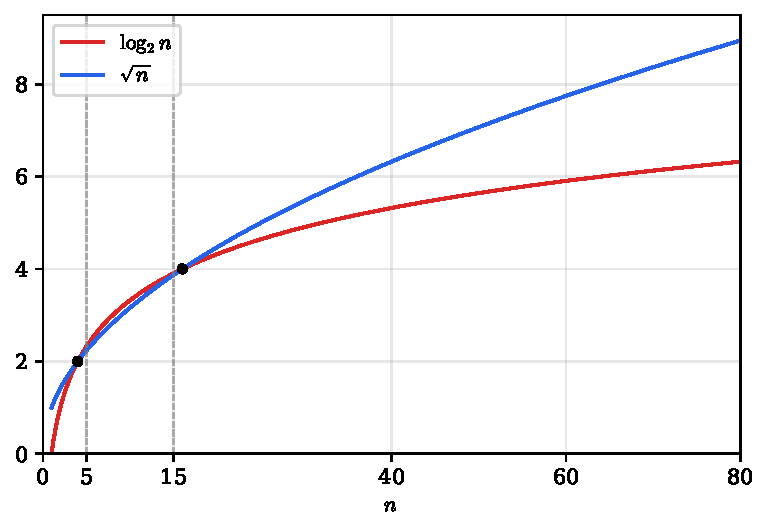
\includegraphics[width=0.75\linewidth]{act2_log_vs_raiz.pdf}
  \caption{$\log_2 n$ y $\sqrt{n}$ para $1 \le n \le 80$. Los puntos marcan los cruces
  en $n = 4$ y $n = 16$, y las líneas rayadas marcan $n = 5$ y $n = 15$, el primer y el
  último entero donde $\log_2 n > \sqrt{n}$. Generada con
  \texttt{scripts/act2\_log\_vs\_raiz.py}.}
  \label{fig:act2-log-vs-raiz}
\end{figure}
Las dos curvas se cruzan en $n = 4$, donde ambas valen $2$, y en $n = 16$, donde ambas
valen $4$. Entre esos dos puntos el logaritmo queda por encima de la raíz, así que la
desigualdad falla para todos los enteros entre $5$ y $15$. Por eso hay que elegir un $n_0$
a partir del cual la desigualdad se cumpla siempre.

Para comparar $\log_2 n$ con $\sqrt{n}$, ubicamos $n$
entre dos potencias de 2 seguidas. Sea $k = \floor{\log_2 n}$, de modo que
\[
  2^k \le n < 2^{k+1}.
\]
De ahí salen dos desigualdades. Aplicando logaritmo a $n < 2^{k+1}$, queda
$\log_2 n < k + 1$. Y sacando raíz a $2^k \le n$, queda $\sqrt{2^k} \le \sqrt{n}$.
Entonces, si mostramos que
\[
  k + 1 \le \sqrt{2^k},
\]
tendremos $\log_2 n < k + 1 \le \sqrt{2^k} \le \sqrt{n}$, que es lo que buscamos. Como
ambos lados son positivos, $k + 1 \le \sqrt{2^k}$ es lo mismo que $(k + 1)^2 \le 2^k$.

Ahora demostramos por inducción que $(k+1)^2 \le 2^k$ para todo $k \ge 6$.
\begin{itemize}
  \item \textbf{Caso base, $k = 6$:} $(6 + 1)^2 = 49 \le 64 = 2^6$.
  \item \textbf{Paso inductivo:} suponemos que $(k+1)^2 \le 2^k$ para algún $k \ge 6$
        (hipótesis de inducción) y mostramos que la desigualdad también vale para $k + 1$.
        Al reemplazar $k$ por $k + 1$, el lado izquierdo $(k+1)^2$ pasa a ser $(k+2)^2$ y
        el lado derecho $2^k$ pasa a ser $2^{k+1}$, así que hay que probar
        \[
          (k+2)^2 \le 2^{k+1}.
        \]
        Escribimos $k + 2$ como $(k+1) + 1$ y desarrollamos el cuadrado de un binomio,
        $(a + 1)^2 = a^2 + 2a + 1$, con $a = k + 1$:
        \[
          (k+2)^2 = \big((k+1) + 1\big)^2 = (k+1)^2 + 2(k+1) + 1 = (k+1)^2 + 2k + 3.
        \]
        El primer término, $(k+1)^2$, es el que aparece en la hipótesis. Ahora acotamos
        el resto, $2k + 3$, por ese mismo término. Restando,
        \[
          (k+1)^2 - (2k+3) = k^2 + 2k + 1 - 2k - 3 = k^2 - 2,
        \]
        y $k^2 - 2 > 0$ para $k \ge 6$ (de hecho, para todo $k \ge 2$). Luego
        $2k + 3 < (k+1)^2$, y reemplazando en la expresión de $(k+2)^2$:
        \[
          (k+2)^2 = (k+1)^2 + (2k + 3) \le (k+1)^2 + (k+1)^2 = 2\,(k+1)^2.
        \]
        Por la hipótesis de inducción, $(k+1)^2 \le 2^k$, y multiplicando por 2 queda
        $2\,(k+1)^2 \le 2 \cdot 2^k = 2^{k+1}$. Juntando las dos desigualdades:
        \[
          (k+2)^2 \le 2\,(k+1)^2 \le 2^{k+1},
        \]
        que es lo que había que probar.
\end{itemize}
Por lo tanto, $(k+1)^2 \le 2^k$ para todo $k \ge 6$. El caso $k = 5$ no sirve, porque
$36 > 32$.

Con esto, si $n \ge 64 = 2^6$, entonces $k = \floor{\log_2 n} \ge 6$, y por
lo anterior
\[
  \log_2 n \le \sqrt{n} \qquad \text{para todo } n \ge 64.
\]
Multiplicando ambos lados por $n$:
\[
  n \log_2 n \le n \sqrt{n} = 1 \cdot n^{3/2}.
\]
Luego, $c = 1$ y $n_0 = 64$. Por lo tanto, $n \log_2 n \in \Oh{n^{3/2}}$.



\section{Actividad 3: Dividir para Conquistar y recurrencias}
\label{sec:act3}

En esta actividad obtenemos la recurrencia de cada algoritmo a partir de su pseudocódigo y
la resolvemos con un árbol de recursión o por sustitución.

\subsection{Árbol de recursión: divisiones de distinto tamaño}
\label{sec:act3-1}

\begin{enunciado}
Considere el siguiente algoritmo:
\begin{lstlisting}[language={}, numbers=none, frame=none, backgroundcolor={}]
Procedure RecursiveFilter(A, n)
    if n <= 1
        return

    for i = 1 to n
        Process(A[i])          // costo Theta(1)

    RecursiveFilter(A[1 ... floor(n/2)], floor(n/2))
    RecursiveFilter(A[1 ... floor(n/4)], floor(n/4))
\end{lstlisting}
\begin{enumerate}[label=(\alph*)]
  \item Formule la recurrencia de tiempo.
  \item Dibuje al menos los primeros tres niveles del árbol de recursión, indicando el
        tamaño de cada subproblema y el trabajo no recursivo de cada nodo.
  \item Determine una cota superior para el trabajo agregado de cada nivel.
  \item Utilizando el árbol, obtenga una cota $\Theta$ para el tiempo total.
  \item Explique por qué la forma estándar del Teorema Maestro no se aplica directamente a
        esta recurrencia.
\end{enumerate}
\end{enunciado}

% ============================================================
\subsubsection*{(a) Recurrencia de tiempo}

Llamamos $T(n)$ al tiempo que tarda \texttt{RecursiveFilter} con un arreglo de tamaño
$n$. Recorremos el pseudocódigo línea por línea.

Si $n \le 1$, el algoritmo solo hace la comparación \texttt{n <= 1} y termina. Eso cuesta
una constante, que llamamos $c$.

Si $n > 1$, el algoritmo primero hace la misma comparación, que cuesta una constante.
Después viene el for, que da $n$ vueltas. En cada vuelta se ejecuta \texttt{Process}, de
costo $\T{1}$, y se avanza el índice, así que el for cuesta $\T{n}$. Al final hay dos
llamadas recursivas: una con un arreglo de tamaño $\floor{n/2}$, que tarda
$T(\floor{n/2})$, y otra con un arreglo de tamaño $\floor{n/4}$, que tarda
$T(\floor{n/4})$. Suponemos que pasar el subarreglo $A[1 \dots k]$ no copia los datos,
sino que solo indica dónde termina, así que cuesta $\T{1}$.
La comparación y el for juntos cuestan a lo más $c\,n$ para alguna constante $c$, que
podemos tomar igual a la del caso base. Entonces:
\[
  T(n) =
  \begin{cases}
    c, & n \le 1, \\[4pt]
    T\!\left(\floor*{\dfrac{n}{2}}\right) + T\!\left(\floor*{\dfrac{n}{4}}\right) + c\,n, & n > 1.
  \end{cases}
\]
El término $T(\floor{n/2})$ viene de la primera llamada recursiva, $T(\floor{n/4})$ de la
segunda, y $c\,n$ del for y la comparación. En adelante omitimos los pisos y escribimos
\[
  T(n) = T\!\left(\frac{n}{2}\right) + T\!\left(\frac{n}{4}\right) + c\,n.
\]
Así los tamaños del árbol quedan como $n/2$, $n/4$, $n/8$, y la suma de cada nivel es
fácil de calcular. Esto no cambia el resultado. El piso solo achica los tamaños, así que
la cota superior que obtenemos sin pisos también vale con ellos, y la cota inferior solo
usa la raíz, que tiene tamaño $n$.

% ============================================================
\subsubsection*{(b) Árbol de recursión}

Cada nodo del árbol es una llamada. Dentro de cada nodo anotamos el tamaño del
subproblema y, debajo, su trabajo no recursivo, que es $c$ por el tamaño. Cada nodo de
tamaño $s$ tiene dos hijos, de tamaños $s/2$ y $s/4$. En la tabla de abajo va la suma de cada
nivel.

\begin{center}
\begin{forest}
  for tree={
    draw, rounded corners, align=center, font=\small,
    l sep=12mm, s sep=4mm, inner sep=3pt, edge={->}
  }
  [{$n$\\[1pt]$c\,n$}
    [{$n/2$\\[1pt]$c\,n/2$}
      [{$n/4$\\[1pt]$c\,n/4$}]
      [{$n/8$\\[1pt]$c\,n/8$}]
    ]
    [{$n/4$\\[1pt]$c\,n/4$}
      [{$n/8$\\[1pt]$c\,n/8$}]
      [{$n/16$\\[1pt]$c\,n/16$}]
    ]
  ]
\end{forest}
\end{center}

\begin{center}
\begin{tabular}{ccl}
  \toprule
  nivel & tamaños de los nodos & trabajo del nivel \\
  \midrule
  0 & $n$ & $c\,n$ \\[2pt]
  1 & $\frac{n}{2},\ \frac{n}{4}$ & $c\left(\frac12 + \frac14\right) n = \frac34\, c\,n$ \\[4pt]
  2 & $\frac{n}{4},\ \frac{n}{8},\ \frac{n}{8},\ \frac{n}{16}$
    & $c\left(\frac14 + \frac18 + \frac18 + \frac1{16}\right) n = \frac{9}{16}\, c\,n
       = \left(\frac34\right)^2 c\,n$ \\
  \bottomrule
\end{tabular}
\end{center}

La rama de más a la izquierda siempre divide por $2$, así que llega a tamaño $1$ después
de $\log_2 n$ niveles. La de más a la derecha siempre divide por $4$, así que llega antes,
después de $\log_4 n$ niveles. Por eso el árbol no es completo: a partir del nivel
$\log_4 n$ algunas ramas ya terminaron.

% ============================================================
\subsubsection*{(c) Cota superior para el trabajo de cada nivel}

En la tabla se ve que el trabajo de cada nivel es $\frac34$ del anterior. La razón es que
un nodo de tamaño $s$ tiene hijos de tamaños $s/2$ y $s/4$, que suman
\[
  \frac{s}{2} + \frac{s}{4} = \frac34\, s.
\]
Es decir, al bajar un nivel, la suma de los tamaños se multiplica por $\frac34$. Como el
trabajo de cada nodo es $c$ por su tamaño, el trabajo del nivel también se multiplica
por $\frac34$. Cuando una rama termina, sus nodos dejan de aparecer en los niveles
siguientes, y el redondeo hacia abajo solo achica los tamaños, así que el trabajo de un
nivel nunca supera ese valor. Por lo tanto, el trabajo del nivel $i$ cumple
\[
  \text{trabajo del nivel } i \le \left(\frac34\right)^{i} c\,n.
\]

% ============================================================
\subsubsection*{(d) Cota $\Theta$ para el tiempo total}

\textbf{Cota superior.} El tiempo total es la suma del trabajo de todos los niveles.
Usando la cota de (c) y dejando que la suma siga para siempre:
\[
  T(n) \le c\,n + \frac34\, c\,n + \left(\frac34\right)^2 c\,n + \cdots
       = c\,n \left( 1 + \frac34 + \left(\frac34\right)^2 + \cdots \right).
\]
Lo que queda entre paréntesis es una serie geométrica de razón $3/4$:
\[
  1 + \frac34 + \left(\frac34\right)^2 + \cdots = \frac{1}{1 - 3/4} = 4.
\]
Reemplazando este valor, el trabajo de los nodos internos es a lo más $4c\,n$.

Falta sumar las hojas, que son las llamadas con $n \le 1$. Se suman aparte porque una
hoja no entra al for. Solo hace la comparación \texttt{n <= 1}, así que cuesta $c$ aunque
su tamaño sea $0$, y la cota de (c), que cuenta $c$ por el tamaño, no la incluye bien.

Cada nodo interno tiene tamaño al menos $2$, así que su trabajo es al menos $2c$. Como el
trabajo de todos los nodos internos suma a lo más $4c\,n$, hay a lo más $2n$ nodos
internos. Cada nodo interno tiene dos hijos, así que hay a lo más $4n$ hojas, y entre
todas cuestan a lo más $4c\,n$. Por lo tanto,
\[
  T(n) \le 4c\,n + 4c\,n = 8c\,n.
\]

\textbf{Cota inferior.} La raíz sola ya hace un trabajo de $c\,n$, y los demás nodos no
pueden restar. Por lo tanto, $T(n) \ge c\,n$.

Juntando ambas cotas:
\[
  c \cdot n \le T(n) \le 8c \cdot n.
\]
Según la definición vista en clases, $T(n) \in \T{n}$ si existen dos constantes
$c_1, c_2 > 0$ y un $n_0 \in \N$ tales que $0 \le c_1 n \le T(n) \le c_2 n$ para todo
$n \ge n_0$. Luego, $c_1 = c$ y $c_2 = 8c$, y las dos cotas valen desde $n = 2$, así que
$n_0 = 2$. Por lo tanto, $T(n) \in \T{n}$.

El trabajo total es del mismo orden que el de la raíz. Como cada nivel hace $\frac34$ del
trabajo del anterior, el trabajo decrece geométricamente y la raíz domina, igual que en
el ejemplo de clases con $T(n) = 3T(n/4) + c\,n^2$.

% ============================================================
\subsubsection*{(e) Por qué no se aplica el Teorema Maestro}

La forma estándar del Teorema Maestro es para recurrencias del tipo
\[
  T(n) = a\, T\!\left(\frac{n}{b}\right) + f(n),
\]
donde los $a$ subproblemas tienen todos el mismo tamaño $n/b$. En nuestra recurrencia hay
dos subproblemas de tamaños distintos, $n/2$ y $n/4$, así que no existe un único $b$ que
la describa. Por eso no se puede comparar $f(n)$ con $n^{\log_b a}$, que es lo que hace
el teorema. Este es justamente uno de los casos que se vieron en clases como
``subproblemas de tamaños distintos'', junto con el ejemplo $T(n/3) + T(2n/3) + n$, que
también se resuelve con el árbol de recursión.


\subsection{Sustitución: construcción simple de un k-d tree}
\label{sec:act3-2}

\begin{enunciado}
Considere una construcción de k-d tree en la cual, en cada llamada recursiva, los puntos
se ordenan por la coordenada correspondiente al nivel, se selecciona la mediana y se
construyen recursivamente ambos subárboles.
\begin{lstlisting}[language={}, numbers=none, frame=none, backgroundcolor={}]
BuildKD(P, depth)
    if |P| <= 1
        return leaf(P)

    axis = depth mod d
    sort P according to coordinate axis
    m = floor(|P|/2)

    node.point = P[m]
    node.left  = BuildKD(P[0 ... m-1], depth+1)
    node.right = BuildKD(P[m+1 ... |P|-1], depth+1)
    return node
\end{lstlisting}
Suponga que ordenar $m$ puntos tiene costo $\T{m \log m}$ y que las particiones quedan
balanceadas.
\begin{enumerate}[label=(\alph*)]
  \item Obtenga la recurrencia correspondiente.
  \item Proponga una cota asintótica para la recurrencia. Puede utilizar un árbol de
        recursión únicamente para formular la conjetura.
  \item Demuestre la cota mediante el método de sustitución. La demostración debe incluir
        cota superior y cota inferior, o una argumentación equivalente que permita concluir
        una cota $\Theta$.
  \item Si en vez de ordenar completamente en cada llamada la mediana pudiera obtenerse y
        particionarse en $\T{m}$, escriba la nueva recurrencia y determine cómo cambiaría
        el costo de construcción.
\end{enumerate}
\end{enunciado}

% ============================================================
\subsubsection*{(a) Recurrencia}

Llamamos $T(n)$ al tiempo que tarda \texttt{BuildKD} con un conjunto $P$ de $n$ puntos.
Recorremos el pseudocódigo línea por línea.

Si $n \le 1$, el algoritmo compara $|P|$ con $1$ y crea una hoja. Eso cuesta una
constante, que llamamos $c$.

Si $n \ge 2$, el algoritmo compara $|P|$ con $1$, calcula \texttt{axis} y \texttt{m}, y
guarda \texttt{node.point}. Cada una de estas operaciones cuesta $\T{1}$. Además ordena
los $n$ puntos según la coordenada \texttt{axis}, lo que según el enunciado cuesta
$\T{n \log n}$. Juntando todo, el trabajo que no es recursivo es $\T{n \log n}$, porque
las operaciones de costo constante quedan absorbidas por el ordenamiento. Al final hay
dos llamadas recursivas: una con los puntos $P[0 \dots m-1]$ y otra con
$P[m+1 \dots |P|-1]$. Como $m = \floor{n/2}$, cada una recibe a lo más $n/2$ puntos, y
como las particiones quedan balanceadas, cada llamada tarda $T(n/2)$. Suponemos que
pasar un subarreglo no copia los puntos, así que cuesta $\T{1}$.

Para no cargar la notación, usamos la misma constante $c$ para el caso base y para el
trabajo no recursivo, que escribimos como $c\,n\log_2 n$. Entonces:
\[
  T(n) =
  \begin{cases}
    c, & n \le 1, \\[4pt]
    2\,T\!\left(\dfrac{n}{2}\right) + c\,n \log_2 n, & n \ge 2.
  \end{cases}
\]
El $2\,T(n/2)$ viene de las dos llamadas recursivas, \texttt{node.left} y
\texttt{node.right}, y el término $c\,n\log_2 n$ viene del ordenamiento. Como se permite
en clases, suponemos que $n$ es una potencia de $2$.

% ============================================================
\subsubsection*{(b) Conjetura con el árbol de recursión}

Usamos el árbol de recursión para formular la conjetura, que luego se demuestra por
sustitución en (c). Cada nodo es una llamada. Dentro de cada
nodo anotamos el tamaño del subproblema y, debajo, su trabajo no recursivo. La raíz tiene
tamaño $n$ y trabajo $c\,n\log_2 n$, y cada nodo de tamaño $s$ tiene dos hijos de tamaño
$s/2$.

\begin{center}
\begin{forest}
  for tree={
    draw, rounded corners, align=center, font=\small,
    l sep=12mm, s sep=3mm, inner sep=3pt, edge={->}
  }
  [{$n$\\[1pt]$c\,n\log_2 n$}
    [{$n/2$\\[1pt]$c\,\frac{n}{2}\log_2\frac{n}{2}$}
      [{$n/4$\\[1pt]$c\,\frac{n}{4}\log_2\frac{n}{4}$}]
      [{$n/4$\\[1pt]$c\,\frac{n}{4}\log_2\frac{n}{4}$}]
    ]
    [{$n/2$\\[1pt]$c\,\frac{n}{2}\log_2\frac{n}{2}$}
      [{$n/4$\\[1pt]$c\,\frac{n}{4}\log_2\frac{n}{4}$}]
      [{$n/4$\\[1pt]$c\,\frac{n}{4}\log_2\frac{n}{4}$}]
    ]
  ]
\end{forest}
\end{center}

En el nivel $i$ hay $2^i$ nodos, cada uno de tamaño $n/2^i$. Los tamaños se dividen por
$2$ en cada nivel, así que llegan a $1$ en el nivel $\log_2 n$, donde están las $n$
hojas. Cada hoja cuesta $c$.
\begin{center}
\begin{tabular}{cccc}
  \toprule
  nivel & nodos & tamaño de cada nodo & trabajo del nivel \\
  \midrule
  0 & $1$   & $n$     & $c\,n \log_2 n$ \\[2pt]
  1 & $2$   & $n/2$   & $2 \cdot c\,\frac{n}{2} \log_2 \frac{n}{2} = c\,n\,(\log_2 n - 1)$ \\[4pt]
  2 & $4$   & $n/4$   & $4 \cdot c\,\frac{n}{4} \log_2 \frac{n}{4} = c\,n\,(\log_2 n - 2)$ \\[2pt]
  $\vdots$ & $\vdots$ & $\vdots$ & $\vdots$ \\
  $i$ & $2^i$ & $n/2^i$ & $c\,n\,(\log_2 n - i)$ \\
  $\vdots$ & $\vdots$ & $\vdots$ & $\vdots$ \\
  $\log_2 n - 1$ & $n/2$ & $2$ & $c\,n \cdot 1$ \\[2pt]
  $\log_2 n$ (hojas) & $n$ & $1$ & $c\,n$ \\
  \bottomrule
\end{tabular}
\end{center}
Sumando los niveles internos, del $0$ al $\log_2 n - 1$, el factor entre paréntesis toma
los valores $\log_2 n, \log_2 n - 1, \dots, 2, 1$:
\[
  c\,n\,\big(\log_2 n + (\log_2 n - 1) + \cdots + 2 + 1\big)
  = c\,n \cdot \frac{\log_2 n\,(\log_2 n + 1)}{2}
  = \frac{c}{2}\, n \log_2^2 n + \frac{c}{2}\, n \log_2 n,
\]
donde usamos la suma $1 + 2 + \cdots + L = L(L+1)/2$ con $L = \log_2 n$. Agregando las
hojas, el árbol suma
\[
  \frac{c}{2}\, n \log_2^2 n + \frac{c}{2}\, n \log_2 n + c\,n.
\]
El término que más crece es $\frac{c}{2}\, n\log_2^2 n$. A diferencia de la Actividad
3.1, el trabajo de los niveles no baja en forma geométrica: baja solo de a $c\,n$ por
nivel, así que la mitad de los niveles cuesta al menos la mitad de lo que cuesta la raíz.
Son $\log_2 n$ niveles que cuestan del orden de $n\log_2 n$ cada uno, y por eso
conjeturamos
\[
  T(n) \in \T{n \log^2 n}.
\]
Es el mismo ejemplo que se vio en clases para la forma general del caso 2 del Teorema
Maestro: $2T(n/2) + n\log n \in \T{n\log^2 n}$.

% ============================================================
\subsubsection*{(c) Demostración por sustitución}

En las dos cotas usamos que, como $n$ es potencia de $2$,
\[
  \log_2 \frac{n}{2} = \log_2 n - 1,
  \qquad \text{y por lo tanto} \qquad
  \left( \log_2 \frac{n}{2} \right)^2 = \log_2^2 n - 2\log_2 n + 1.
\]

\textbf{Cota superior.} Conjetura: $T(n) \le 2c\, n \log_2^2 n$ para todo $n \ge 2$.

\emph{Caso base, $n = 2$.} Por la recurrencia, $T(2) = 2\,T(1) + c \cdot 2 \cdot \log_2 2$.
Como $T(1) = c$ y $\log_2 2 = 1$, queda $T(2) = 2c + 2c = 4c$. La cota en $n = 2$ vale
$2c \cdot 2 \cdot (\log_2 2)^2 = 4c$, así que se cumple $4c \le 4c$. Este caso también
explica la constante. Si la conjetura fuera $T(n) \le d\, n\log_2^2 n$, en $n = 2$ se
necesitaría $4c \le 2d$, es decir, $d \ge 2c$, y tomamos el menor valor posible,
$d = 2c$.

La base no puede ser $n = 1$, porque ahí la cota vale $2c \cdot 1 \cdot (\log_2 1)^2 = 0$
y $T(1) = c$ es mayor que $0$. La cota es falsa en $n = 1$, y por eso la conjetura se
plantea desde $n = 2$. Partir de $n = 2$ alcanza para cubrir todos los casos. Como $n$ es
potencia de $2$, los valores que importan son $2, 4, 8, 16, \dots$, y cada uno es el doble
del anterior. El paso inductivo lleva la cota de $n/2$ a $n$, así que desde $n = 2$ se
llega a $4$, de $4$ a $8$, y así sucesivamente. El paso parte en $n = 4$ para que $n/2$
sea al menos $2$ y la hipótesis se pueda usar.

\emph{Paso inductivo.} Sea $n \ge 4$ y supongamos que la cota vale para $n/2$, es decir,
$T(n/2) \le 2c\, \frac{n}{2} \log_2^2 \frac{n}{2}$. Sustituyendo en la recurrencia:
\[
\begin{aligned}
  T(n) &= 2\,T\!\left(\frac{n}{2}\right) + c\,n\log_2 n \\
       &\le 2 \cdot 2c\, \frac{n}{2} \left(\log_2 n - 1\right)^2 + c\,n\log_2 n \\
       &= 2c\,n \left(\log_2^2 n - 2\log_2 n + 1\right) + c\,n\log_2 n \\
       &= 2c\,n\log_2^2 n - 3c\,n\log_2 n + 2c\,n.
\end{aligned}
\]
Para que esto sea a lo más $2c\,n\log_2^2 n$, lo que sobra tiene que ser negativo o cero:
$-3c\,n\log_2 n + 2c\,n \le 0$. Dividiendo por $c\,n$, eso es $3\log_2 n \ge 2$, que se
cumple porque $\log_2 n \ge 2$ para $n \ge 4$. Por lo tanto, $T(n) \le 2c\,n\log_2^2 n$
con la misma constante, como exige el método.

\textbf{Cota inferior.} Conjetura: $T(n) \ge \frac{c}{2}\, n \log_2^2 n$ para todo $n \ge 1$.

\emph{Caso base, $n = 1$.} $T(1) = c$, y la cota vale
$\frac{c}{2} \cdot 1 \cdot 0 = 0$. Se cumple $c \ge 0$.

\emph{Paso inductivo.} Sea $n \ge 2$ y supongamos que la cota vale para $n/2$. Sustituyendo:
\[
\begin{aligned}
  T(n) &= 2\,T\!\left(\frac{n}{2}\right) + c\,n\log_2 n \\
       &\ge 2 \cdot \frac{c}{2}\, \frac{n}{2} \left(\log_2 n - 1\right)^2 + c\,n\log_2 n \\
       &= \frac{c}{2}\, n \left(\log_2^2 n - 2\log_2 n + 1\right) + c\,n\log_2 n \\
       &= \frac{c}{2}\, n\log_2^2 n + \frac{c}{2}\, n.
\end{aligned}
\]
Como $\frac{c}{2}\, n \ge 0$, queda $T(n) \ge \frac{c}{2}\, n\log_2^2 n$ con la misma
constante.

Juntando ambas cotas, para todo $n \ge 2$:
\[
  \frac{c}{2} \cdot n\log_2^2 n \le T(n) \le 2c \cdot n\log_2^2 n.
\]
Según la definición vista en clases, $T(n) \in \T{n\log^2 n}$ si existen dos constantes
$c_1, c_2 > 0$ y un $n_0 \in \N$ tales que $0 \le c_1 n\log_2^2 n \le T(n) \le c_2 n\log_2^2 n$
para todo $n \ge n_0$. Luego, $c_1 = c/2$ y $c_2 = 2c$, y las dos cotas valen desde
$n = 2$, así que $n_0 = 2$. Por lo tanto, $T(n) \in \T{n \log^2 n}$.

% ============================================================
\subsubsection*{(d) Mediana en tiempo lineal}

Si la mediana se pudiera obtener y los puntos se pudieran particionar en $\T{n}$, el
único cambio estaría en el trabajo no recursivo: el ordenamiento, de costo $\T{n\log n}$,
se reemplaza por una operación de costo $\T{n}$. Las dos llamadas recursivas siguen igual.
La nueva recurrencia es
\[
  T(n) = 2\,T\!\left(\frac{n}{2}\right) + c\,n.
\]
Es la misma recurrencia de Merge Sort, que se resolvió en clases: cada nivel del árbol
cuesta $c\,n$ y hay $\log_2 n + 1$ niveles, así que
\[
  T(n) \in \T{n\log n}.
\]
El costo de construcción baja de $\T{n\log^2 n}$ a $\T{n\log n}$, es decir, se ahorra un
factor $\log n$. Ese factor venía de ordenar en cada llamada, cuando para elegir la
mediana no hace falta ordenar todo. Una forma de lograrlo es el algoritmo de selección
con mediana de medianas, cuya recurrencia $T(n/5) + T(7n/10) + n$ se vio en clases y da
$\T{n}$.



\section{Actividad 4: k-d tree para clasificación 1-NN}
\label{sec:act4}


En esta actividad implementamos un k-d tree, construido con Dividir para Conquistar, y
lo usamos para clasificar dígitos manuscritos con 1-NN. Comparamos su búsqueda exacta del
vecino más cercano con la búsqueda exhaustiva para distintas dimensionalidades,
obtenidas con PCA, y observamos cómo esa reducción afecta la clasificación.

El código está en el repositorio: \texttt{src/kdtree.py} tiene la estructura y las dos
búsquedas, y \texttt{scripts/act4\_kdtree.py} ejecuta los experimentos y genera las
tablas y figuras de esta sección, con el comando \texttt{python scripts/act4\_kdtree.py}.

% ============================================================
\subsection{Implementación}

\textbf{Distancia.} Las dos estrategias usan la misma función para la distancia euclidiana
al cuadrado, escrita con el mismo ciclo del enunciado:
\begin{lstlisting}
def squared_distance(a, b):
    suma = 0.0
    for j in range(len(a)):
        diff = a[j] - b[j]
        suma = suma + diff * diff
    return suma
\end{lstlisting}

\textbf{Estructura.} Cada nodo es un diccionario que guarda un punto, su posición en el
conjunto de entrenamiento, el eje de partición y referencias a sus dos hijos.

\textbf{Construcción.} Es la aplicación de Dividir para Conquistar de esta actividad. En
cada llamada se elige el eje como \texttt{depth mod d}, se ordenan los puntos según ese
eje, se toma la mediana $m = \floor{n/2}$ como nodo y se construyen recursivamente los dos
subárboles, con los puntos a la izquierda y a la derecha de la mediana. Es el algoritmo de
la Actividad 3.2, así que la construcción cuesta $\T{n\log^2 n}$. Como la mediana divide
los puntos en dos mitades, el árbol queda balanceado y tiene altura
$\floor{\log_2 n} + 1$. Con los $1437$ puntos de entrenamiento, eso son $11$ niveles.

\textbf{Búsqueda exacta.} Sigue el esquema del enunciado:
\begin{lstlisting}
def buscar(nodo, q, mejor):
    # `mejor` guarda el mejor vecino encontrado y los nodos visitados.
    if nodo is None:
        return

    mejor["visitados"] = mejor["visitados"] + 1
    dist = squared_distance(q, nodo["punto"])
    if dist < mejor["dist"]:
        mejor["dist"] = dist
        mejor["indice"] = nodo["indice"]

    eje = nodo["eje"]
    delta = q[eje] - nodo["punto"][eje]
    if delta < 0:
        cerca = nodo["izquierdo"]
        lejos = nodo["derecho"]
    else:
        cerca = nodo["derecho"]
        lejos = nodo["izquierdo"]

    buscar(cerca, q, mejor)
    if delta * delta < mejor["dist"]:
        buscar(lejos, q, mejor)
\end{lstlisting}
Primero se visita el subárbol del lado de la consulta. El otro se explora solo si
$\delta^2$, la distancia al cuadrado de la consulta al hiperplano de corte, es menor que
la mejor distancia encontrada. Esa prueba se hace después de explorar el lado cercano,
porque ahí la mejor distancia puede haber bajado. La poda no pierde el vecino exacto:
todos los puntos del otro lado están al menos a distancia $|\delta|$ de la consulta, así
que si $\delta^2$ ya no es menor que la mejor distancia, ninguno de ellos puede mejorarla.
Cada nodo visitado evalúa exactamente una distancia, así que el número de nodos visitados
es también el número de distancias evaluadas.

\textbf{Búsqueda exhaustiva.} Recorre los $n_{\text{train}}$ puntos y se queda con el de
menor distancia, así que evalúa exactamente $n_{\text{train}}$ distancias por consulta.

\textbf{Comparación justa.} Las dos búsquedas están escritas en Python puro, trabajan
sobre los mismos datos (listas de números) y usan la misma \texttt{squared\_distance}. No
se usa NumPy ni ninguna operación vectorizada en ninguna de las dos. Así, la diferencia de
tiempo refleja principalmente cuántas distancias evalúa cada estrategia.

% ============================================================
\subsection{Protocolo experimental}

Usamos el conjunto \texttt{digits} de scikit-learn: $1797$ imágenes de $8 \times 8$
píxeles, con $64$ características y etiquetas de $0$ a $9$. Los datos se separan en
80\,\% entrenamiento ($1437$ imágenes) y 20\,\% prueba ($360$ imágenes), de forma
estratificada y con \texttt{random\_state=42}. Las características se estandarizan con la
media y la desviación del conjunto de entrenamiento, y luego se aplica PCA, ajustado
también solo con entrenamiento, para obtener $d \in \{2, 4, 8, 16, 32\}$ componentes.
scikit-learn se usa únicamente para estos pasos y para la accuracy.

Para cada $d$ se construye el k-d tree sobre los datos de entrenamiento y se clasifican las
$360$ imágenes de prueba con las dos búsquedas. Cada tiempo es la mediana de $7$
repeticiones, y no incluye la carga de datos, la estandarización ni PCA. Como referencia,
agregamos una fila con las $64$ componentes (marcada con $^{*}$), que tiene la misma
geometría que los datos sin reducir. Los experimentos se ejecutaron en un computador con
procesador Apple M2, Python 3.12.2 y scikit-learn 1.6.1.

% ============================================================
\subsection{Correctitud y accuracy}

\begin{table}[H]
  \centering
  \caption{Validación del k-d tree con la búsqueda exhaustiva como referencia, y accuracy
  1-NN en el conjunto de prueba.}
  \small
  \begin{tabular}{crrrr}
\toprule
$d$ & accuracy exhaustiva & accuracy k-d tree & misma distancia mínima & mismo vecino \\
\midrule
2 & 0{,}4472 & 0{,}4472 & 100{,}0\,\% & 100{,}0\,\% \\
4 & 0{,}8056 & 0{,}8056 & 100{,}0\,\% & 100{,}0\,\% \\
8 & 0{,}9306 & 0{,}9306 & 100{,}0\,\% & 100{,}0\,\% \\
16 & 0{,}9583 & 0{,}9583 & 100{,}0\,\% & 100{,}0\,\% \\
32 & 0{,}9722 & 0{,}9722 & 100{,}0\,\% & 100{,}0\,\% \\
64$^{*}$ & 0{,}9667 & 0{,}9667 & 100{,}0\,\% & 100{,}0\,\% \\
\bottomrule
\end{tabular}

\end{table}

Para todas las dimensiones, el k-d tree encuentra la misma distancia mínima y el mismo
vecino que la búsqueda exhaustiva en el 100\,\% de las consultas. No hubo empates, así
que el vecino también coincide siempre. Por eso las dos estrategias tienen exactamente la
misma accuracy.

% ============================================================
\subsection{Resultados}

\begin{table}[H]
  \centering
  \caption{Tiempos (mediana de 7 repeticiones) y speedup de consulta
  $S = T_{\text{exhaustiva}} / T_{\text{k-d tree}}$.}
  \resizebox{\linewidth}{!}{\begin{tabular}{crrrrrr}
\toprule
$d$ & construcción (ms) & exhaustiva total (s) & exhaustiva / consulta (ms) & k-d tree total (s) & k-d tree / consulta (ms) & speedup $S$ \\
\midrule
2 & 4{,}6 & 0{,}085 & 0{,}237 & 0{,}002 & 0{,}006 & 38{,}85 \\
4 & 2{,}7 & 0{,}115 & 0{,}320 & 0{,}008 & 0{,}022 & 14{,}57 \\
8 & 2{,}4 & 0{,}175 & 0{,}487 & 0{,}039 & 0{,}109 & 4{,}46 \\
16 & 3{,}3 & 0{,}285 & 0{,}792 & 0{,}133 & 0{,}368 & 2{,}15 \\
32 & 2{,}4 & 0{,}559 & 1{,}552 & 0{,}313 & 0{,}868 & 1{,}79 \\
64$^{*}$ & 2{,}4 & 1{,}001 & 2{,}781 & 0{,}735 & 2{,}041 & 1{,}36 \\
\bottomrule
\end{tabular}
}
\end{table}

\begin{table}[H]
  \centering
  \caption{Trabajo por consulta: nodos visitados por el k-d tree, fracción del conjunto de
  entrenamiento ($n_{\text{train}} = 1437$) y distancias evaluadas en total por cada
  método para las $360$ consultas.}
  \resizebox{\linewidth}{!}{\begin{tabular}{crrrrrr}
\toprule
$d$ & visitados (promedio) & visitados (mediana) & fracción visitada & $1/\text{fracción}$ & distancias exhaustiva & distancias k-d tree \\
\midrule
2 & 17{,}2 & 16 & 0{,}012 & 83{,}5 & 517\,320 & 6\,199 \\
4 & 53{,}8 & 45 & 0{,}037 & 26{,}7 & 517\,320 & 19\,372 \\
8 & 209{,}2 & 158 & 0{,}146 & 6{,}9 & 517\,320 & 75\,296 \\
16 & 492{,}3 & 373 & 0{,}343 & 2{,}9 & 517\,320 & 177\,239 \\
32 & 737{,}4 & 656 & 0{,}513 & 1{,}9 & 517\,320 & 265\,475 \\
64$^{*}$ & 955{,}5 & 891 & 0{,}665 & 1{,}5 & 517\,320 & 343\,970 \\
\bottomrule
\end{tabular}
}
\end{table}

\begin{figure}[H]
  \centering
  \begin{subfigure}{0.49\linewidth}
    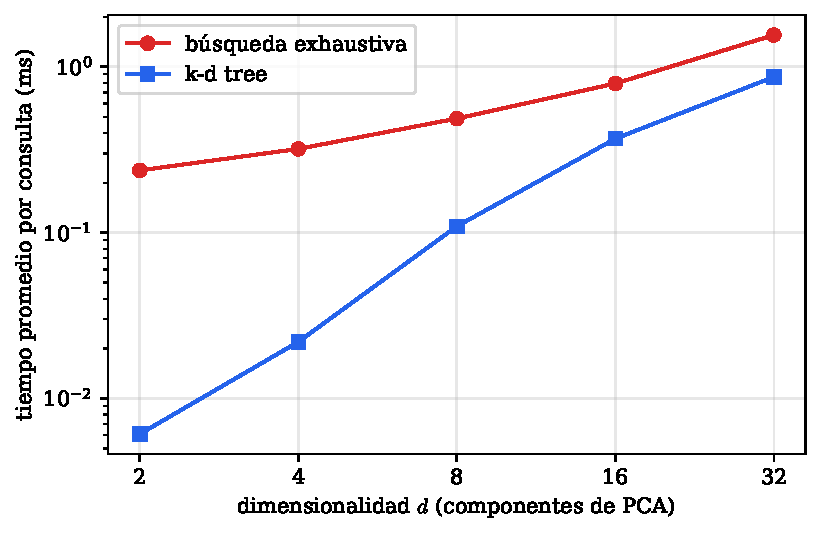
\includegraphics[width=\linewidth]{act4_tiempo_consulta.pdf}
    \caption{Tiempo promedio por consulta.}
  \end{subfigure}\hfill
  \begin{subfigure}{0.49\linewidth}
    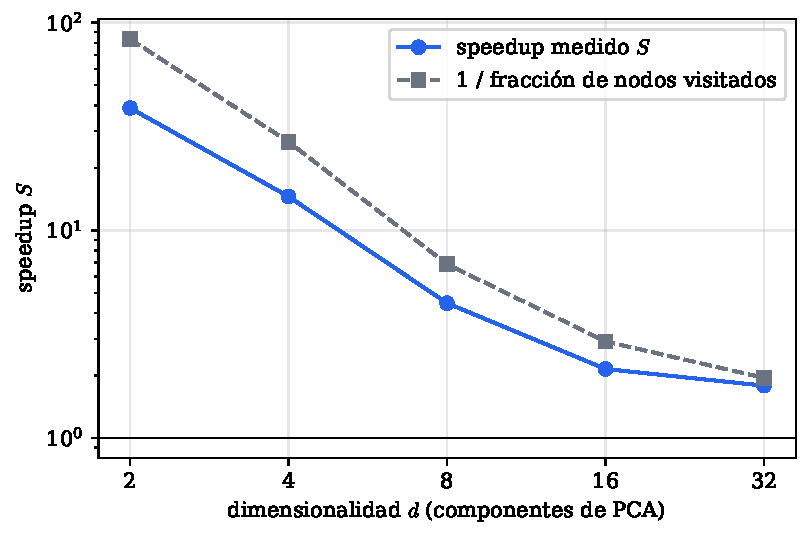
\includegraphics[width=\linewidth]{act4_speedup.pdf}
    \caption{Speedup y $1/\text{fracción visitada}$.}
  \end{subfigure}

  \medskip
  \begin{subfigure}{0.49\linewidth}
    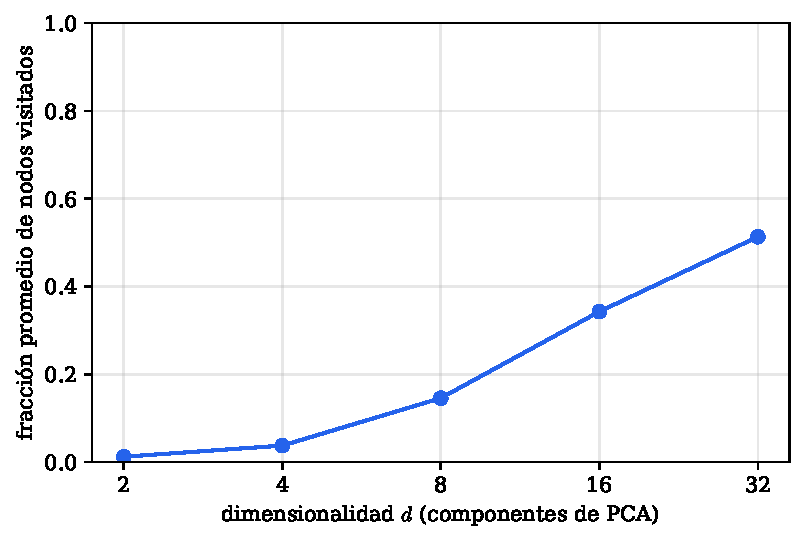
\includegraphics[width=\linewidth]{act4_fraccion_visitada.pdf}
    \caption{Fracción promedio de nodos visitados.}
  \end{subfigure}\hfill
  \begin{subfigure}{0.49\linewidth}
    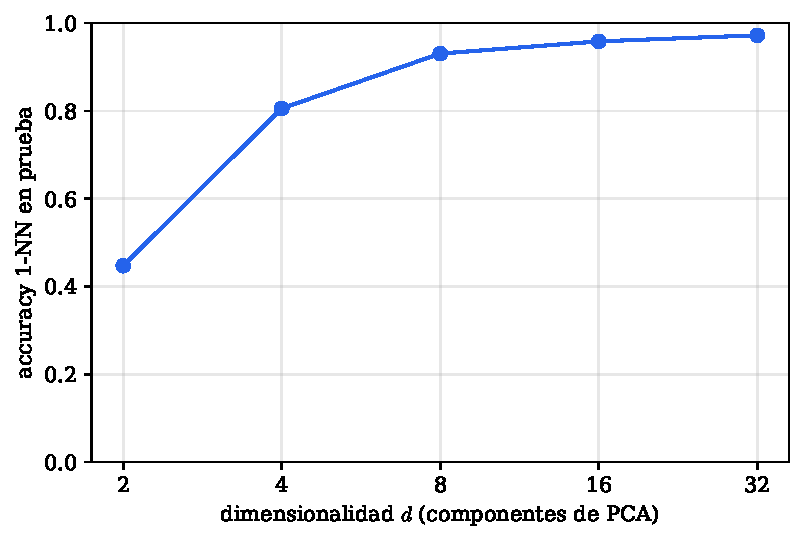
\includegraphics[width=\linewidth]{act4_accuracy.pdf}
    \caption{Accuracy 1-NN.}
  \end{subfigure}
  \caption{Resultados en función de la dimensionalidad $d$. Los ejes horizontales están en
  escala logarítmica, y los verticales de (a) y (b) también.}
\end{figure}

\begin{figure}[H]
  \centering
  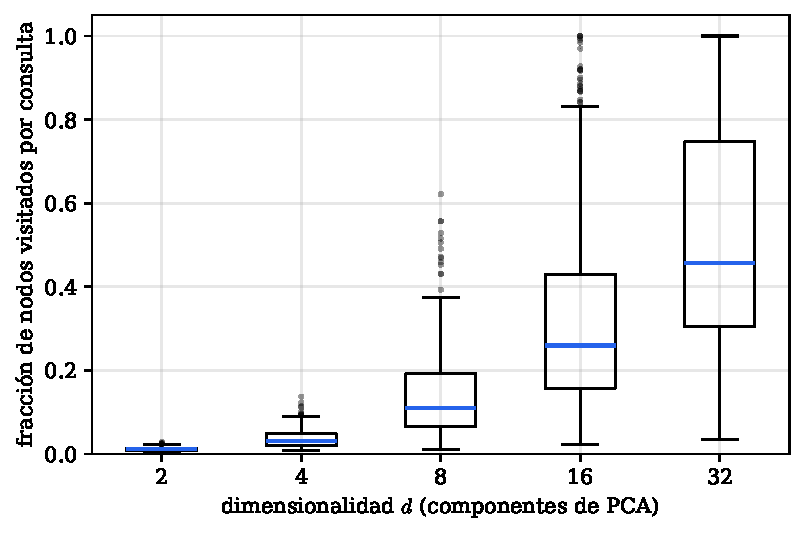
\includegraphics[width=0.7\linewidth]{act4_visitados_distribucion.pdf}
  \caption{Distribución de la fracción de nodos visitados por consulta. Cada caja va del
  primer al tercer cuartil y la línea interior es la mediana.}
\end{figure}

El tiempo de construcción es de unos pocos milisegundos y casi no cambia con $d$, porque
el ordenamiento en cada llamada compara una sola coordenada, sin importar cuántas tenga
cada punto. Con la búsqueda exhaustiva, en cambio, el tiempo por consulta crece con $d$,
porque cada una de las $1437$ distancias recorre $d$ coordenadas.

% ============================================================
\subsection{Discusión}

\textbf{(a) ¿Para qué valores de $d$ el k-d tree reduce claramente el trabajo y el
tiempo?} Para $d = 2$ y $d = 4$ la reducción es grande: el árbol visita cerca del 1\,\% y
del 4\,\% de los puntos, y es unas $39$ y $15$ veces más rápido que la búsqueda
exhaustiva. Con $d = 8$ la ganancia sigue siendo clara: visita cerca del 15\,\% y es unas
$4{,}5$ veces más rápido. Desde $d = 16$ la ganancia es pequeña, de cerca de $2$ veces, y
con $d = 32$ baja a $1{,}8$.

El speedup sigue de cerca al inverso de la fracción de nodos visitados, como se ve en el
gráfico (b). Esto es lo esperable, porque las dos estrategias pagan lo mismo por cada
distancia: si el árbol evalúa la décima parte de las distancias, debería tardar cerca de
la décima parte. El speedup queda algo por debajo de ese valor porque cada nodo visitado
tiene un costo extra que la búsqueda exhaustiva no tiene: la llamada recursiva, el cálculo
de $\delta$ y la decisión de qué lado explorar. Ese costo extra pesa más cuando $d$ es
pequeño, porque ahí una distancia es barata de calcular. Con $d = 2$ el árbol evalúa unas
$83$ veces menos distancias, pero es unas $39$ veces más rápido.

\textbf{(b) ¿Qué ocurre con la fracción de nodos visitados cuando aumenta $d$?} Crece de
forma sostenida: cerca de 1\,\%, 4\,\%, 15\,\%, 34\,\% y 51\,\% para
$d = 2, 4, 8, 16$ y $32$, y llega a 66\,\% con las $64$ componentes. Con más dimensiones,
la distancia de la consulta a cada hiperplano de corte, que mide una sola coordenada, es
pequeña comparada con la distancia al mejor vecino, que suma las diferencias en todas las
coordenadas. Por eso la condición $\delta^2 <$ \texttt{bestDist} se cumple más seguido y
hay que revisar más subárboles. Además, el árbol tiene solo $11$ niveles, así que con
$d = 16$ o $d = 32$ cada camino de la raíz a una hoja corta por a lo más $11$ coordenadas
distintas, y el resto nunca se usa para descartar regiones.

\textbf{(c) ¿Son consistentes los resultados con un peor caso $\Theta(n)$?} Sí. Con
$d = 16$ y $d = 32$ hay consultas que visitan los $1437$ nodos del árbol, es decir, que
hacen el mismo trabajo que la búsqueda exhaustiva, y con $d = 32$ la mediana de nodos
visitados ya es casi la mitad del conjunto. La búsqueda es exacta, y cuando la poda no
logra descartar regiones, termina revisando todos los puntos. El k-d tree no garantiza un
costo logarítmico por consulta: su ventaja depende de la dimensionalidad y de cómo están
distribuidos los datos.

\textbf{(d) ¿Hay relación entre reducir la dimensión con PCA y la accuracy?} Sí. La
accuracy sube de cerca de $0{,}45$ con $d = 2$ a $0{,}81$ con $d = 4$, $0{,}93$ con
$d = 8$, $0{,}96$ con $d = 16$ y $0{,}97$ con $d = 32$. Con pocas componentes se pierde
información que distingue unos dígitos de otros, y el vecino más cercano en ese espacio
reducido muchas veces es de otra clase. Con las $64$ componentes la accuracy es levemente
menor que con $32$, así que más dimensiones no siempre ayudan: las últimas componentes
aportan poca información y algo de ruido.

Esta variación viene de la representación de los datos y no de la búsqueda. Para cada $d$,
el k-d tree y la búsqueda exhaustiva encuentran el mismo vecino en todas las consultas, y
por eso tienen exactamente la misma accuracy. Lo que cambia al variar $d$ es el espacio en
que se miden las distancias, y con él cuál es el vecino más cercano. Esto deja un
compromiso: reducir la dimensión acelera mucho el k-d tree, pero empeora la
clasificación. En este conjunto, $d = 8$ parece un buen punto intermedio, con una accuracy
de $0{,}93$ y una búsqueda unas $4{,}5$ veces más rápida.

\textbf{(e) ¿Por qué el análisis asintótico y la medición experimental se complementan?}
El análisis asintótico describe cómo crece el costo con $n$ y da garantías para cualquier
entrada: la construcción es $\T{n\log^2 n}$ y una consulta exacta puede costar $\T{n}$ en
el peor caso. Pero oculta las constantes y no dice cuánto se poda con unos datos
concretos. La medición muestra el costo real con estos datos, este $n$ y este computador,
incluido el costo extra de la recursión, y permite ver que el caso típico está muy lejos
del peor caso cuando $d$ es pequeño. A su vez, la medición sola no permite generalizar a
otros tamaños o conjuntos de datos, y sus tiempos dependen del hardware. Por eso ninguna
de las dos reemplaza a la otra.



\section*{Declaración de uso de inteligencia artificial}
\addcontentsline{toc}{section}{Declaración de uso de inteligencia artificial}
\label{sec:declaracion-ia}

En este trabajo usamos herramientas de inteligencia artificial generativa con dos fines.
El primero fue revisar las demostraciones, para detectar pasos incompletos o errores en
los cálculos y en las justificaciones. El segundo fue crear el informe en LaTeX, es decir,
dar formato al documento, a las tablas, a las ecuaciones y a los diagramas.

Los planteamientos, los resultados y las conclusiones fueron realizados y revisados por los
integrantes del grupo, que asumen la responsabilidad por el contenido del informe.


\end{document}
